
%(BEGIN_QUESTION)
% Copyright 2008, Tony R. Kuphaldt, released under the Creative Commons Attribution License (v 1.0)
% This means you may do almost anything with this work of mine, so long as you give me proper credit

The following electric heater seems to have a problem: it heats up slower than usual with all three switches turned ``on.''

$$\includegraphics[width=15.5cm]{i03162x01.eps}$$

With three differently-sized heating elements (200 watt, 400 watt, and 800 watt), the oven operator can set the power in seven discrete steps by turning on specific combinations of switches: 200 watts, 400 watts, 600 watts, 800 watts, 1000 watts, 1200 watts, and 1400 watts.

You are summoned to diagnose this oven's problem {\it without turning it off}.  You are allowed to turn off any single switch for a few seconds at most, but otherwise you need to leave all three heaters on because the oven needs to heat up as fast as it can!  The idea is to figure out where the problem might be, then gather together any parts necessary for repairs while the oven is still being used, and fix the oven as fast as possible when you finally get the chance to turn it off completely.

\vskip 10pt

First, assess whether or not the following diagnostic test would provide any useful information about the fault: {\it suppose a technician connects an AC voltmeter between terminals 4 and 8}.  Will this test provide information to help us diagnose the nature and/or location of the fault?  Why or why not?

\vskip 30pt

Next, propose a diagnostic test that would definitely provide useful information about either the location or the nature of the fault in this system.  Your proposal must identify the meaning of at least one possible result of the test (e.g. {\it ``If I jumper terminals $X$ and $Y$ together and I measure a decrease in source voltage, it means the fault must be a short somewhere in branch A-B-C of the circuit''}).  Remember that the best diagnostic test is one that yields definitive answers no matter what its result might be.  Directly checking a suspected component is {\it not} a good diagnostic test, unless there are simply no other options!


\vfil 

\underbar{file i03162}
\eject
%(END_QUESTION)





%(BEGIN_ANSWER)

This is a graded question -- no answers or hints given!

%(END_ANSWER)





%(BEGIN_NOTES)

Measuring voltage between terminals 4 and 8 merely checks the voltage drop across the fuse.  Since we know that the furnace is heating up (albeit slower than we would like), we know for a fact that the fuse cannot be blown.  If the fuse is not blown, it's unlikely it is a contributing factor to the slow heating of the oven, and therefore this diagnostic test is not a good one.

\vskip 10pt

\noindent
More useful diagnostic tests include the following:

\item{} Measure voltage drop across 800 W toggle switch while momentarily turning it off
\item{} Measure voltage drop across 400 W toggle switch while momentarily turning it off
\item{} Measure voltage drop across 200 W toggle switch while momentarily turning it off
\item{} Measure total current (using a clamp-on ammeter) while momentarily turning off the 800 W switch
\item{} Measure total current (using a clamp-on ammeter) while momentarily turning off the 400 W switch
\item{} Measure total current (using a clamp-on ammeter) while momentarily turning off the 200 W switch
\end{itemize}

With any of these proposed tests, what we are doing is seeing whether or not the branch in question has an ``open'' fault, which is a likely cause of the slow heating we're experiencing with this oven.  The kind of voltage measurement indicating a conductive heater branch circuit is one where there is little or no voltage drop when the switch is on, and 240 VAC when the switch is off.  Likewise, the kind of current measurement indicating a conductive heater branch circuit is one where there is a decrease in current when the switch is turned off.

%INDEX% Troubleshooting review: electric circuits

%(END_NOTES)


